\documentclass[aspectratio=43]{beamer}
% \documentclass[aspectratio=169]{beamer} % proyector 16:9 | Ref:  https://en.wikibooks.org/wiki/LaTeX/Presentations
\usetheme{Boadilla}
\beamertemplatenavigationsymbolsempty %% Sin barra navegación
\usecolortheme{beaver}


%% Spanska!
\usepackage[utf8]{inputenc}
\usepackage{lmodern} % no producia letras en matemático | Ref: https://tex.stackexchange.com/questions/250413/error-when-using-greek-symbol-in-subscript-in-beamer-presentation 
\usepackage[spanish]{babel}
\def\spanishoptions{argentina}

%% inclusión de gráficas
\usepackage{graphicx}	% instalar ghostscript-x para que el dvi muestre los eps
\graphicspath{ {./graphs/} {../figuras/} }
\usepackage{rotating}	% epígrafe rotado


\begin{document}

\title{Curso de ingeniería centrado en código}
\subtitle{Experiencia adquirida como legado de la pandemia}
\author[vbettachini@unlam.edu.ar]{Bettachini, V.A.}
\institute[]{
	Ingeniería Mecánica, DIIT, UNLaM
}
\date[2023-09-22]{
	V Encuentro \emph{Mejora de las Estratégias Pedagógicas}\\22 de septiembre de 2023
}

\usebackgroundtemplate{
  
\includegraphics[width=\paperwidth, height=\paperheight]{diit_titre_background}
}	% unset background % https://tex.stackexchange.com/questions/201013/how-to-include-a-background-image-to-only-one-page-of-a-beamer-presentation

\begin{frame} 
  \titlepage
\end{frame}

\usebackgroundtemplate{
  
\includegraphics[width=\paperwidth, height=\paperheight]{diit_background}
} %% https://mprnotes.wordpress.com/2009/08/14/changing-background-image-of-latex-beamer/


\begin{frame}
	\frametitle{Adquisición de competencias: un ejercicio del \emph{copy \& paste}}
	\begin{block}{}
	  \begin{columns}[b]
			\begin{column}{0.3\textwidth}
				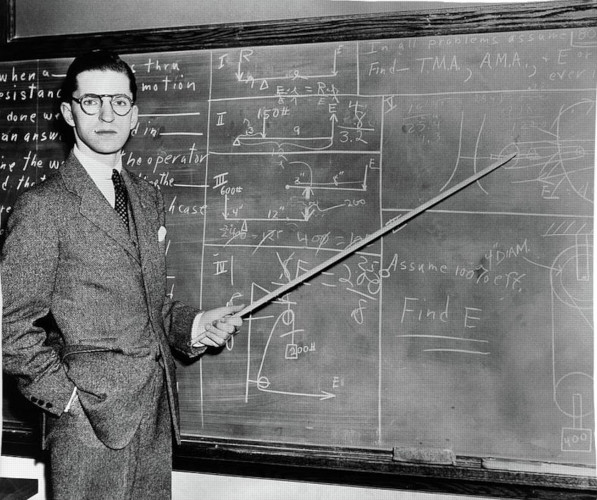
\includegraphics[width= \columnwidth]{1930s-1940s-man-teacher-professor-vintage-images}
			\end{column}
			\begin{column}{0.65\textwidth}
				s. XIX: únicas herramientas pizarrón + papel
				\pause
				\begin{itemize}[<+->]
					% \item Alumnos y docentes pierden tiempo (y se aburren) copiando una y otra vez las mismas cosas
					\item Profesor: \textbf{cada} clase transcribe (o presenta)
					% 	teoría y ejemplos de resolución al 
					\item Alumno: pizarrón (\emph{Powerpoint}) \(\rightarrow\) cuaderno
					\item Modelado y cálculos: \textbf{vuelven} a hacerse
					\item Resuelto en papel \(\implies\) debe \textbf{transcribirse}
				\end{itemize}
			\end{column}
		\end{columns}
	\end{block}

	\pause
	\begin{block}{}
	  \begin{columns}[b]
			\begin{column}{0.3\textwidth}
				\includegraphics[width= \columnwidth]{"Screenshot 2023-09-18 at 12-24-03 Google Colaboratory"}
			\end{column}
			\begin{column}{0.65\textwidth}
				s. XXI: minimizar el tedio del \emph{c\&p}
				\begin{itemize}[<+->]
					% \item Alumnos y docentes pierden tiempo (y se aburren) copiando una y otra vez las mismas cosas
					\item Profesor: actualiza código en repositorio
					\item Alumno: repositorio del curso \(\rightarrow\) propio
					\item Modelado y cálculos: \textbf{única vez}
					\item Código provisto \(\implies\) es \textbf{re-utilizable} 
				\end{itemize}
			\end{column}
		\end{columns}
	\end{block}
\end{frame}



\begin{frame}
	\frametitle{s.XXI: todo el material disponible en línea}
	\pause
	\begin{block}{Cuaderno Jupyter: texto + ecuaciones + código}
		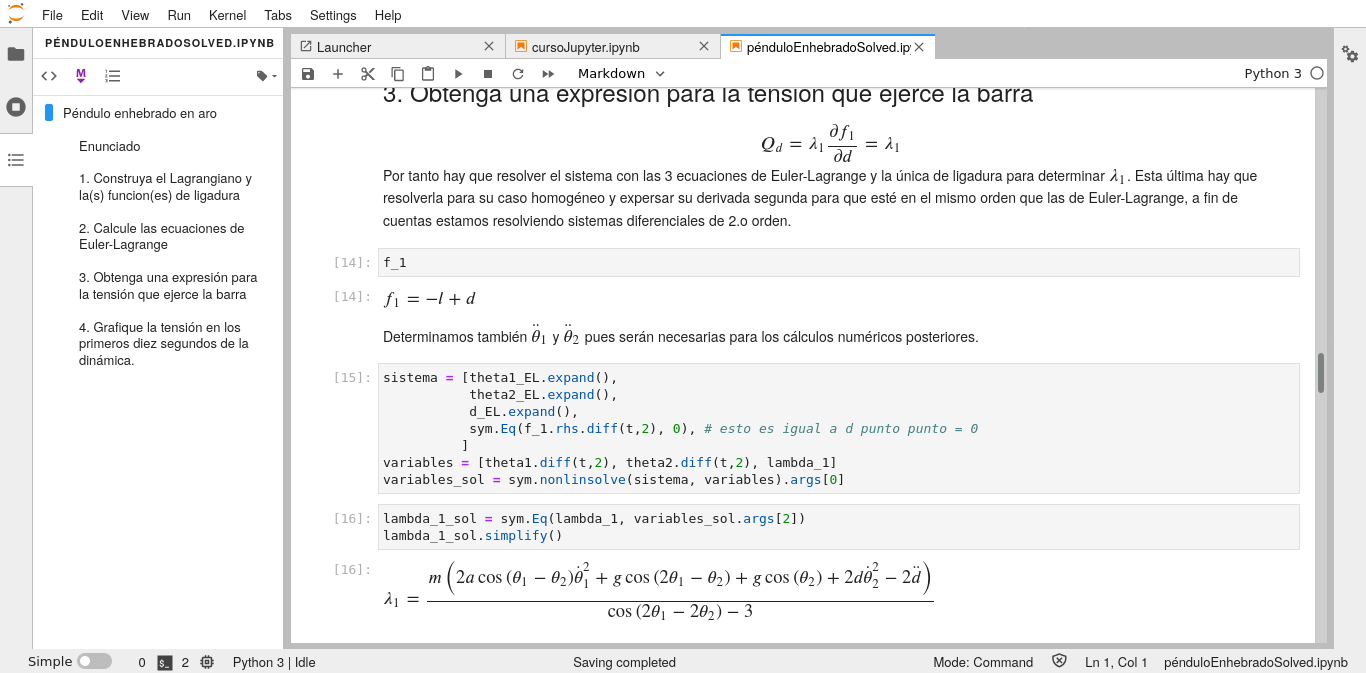
\includegraphics[width= \columnwidth]{screenshot_JupyterLab}
	\end{block}
\end{frame}


\begin{frame}
	\frametitle{¿Por qué formar con código en ingenierías no informáticas?}
	\pause
	\begin{block}{}
		\begin{itemize}[<+->]
			\item Calculadora de bolsillo \(\rightarrow\) \textbf{no repetir} aritmética de primaria.
			\item Sistema de álgebra computacional 
			\begin{itemize}[<+->]
				\item \(\rightarrow\) \textbf{no repetir} asignaturas de álgebra y análisis matemático.\\
				Enfocarse en nuevas habilidades, no en cálculos automatizables.
				\item El cálculo numérico resuelve lo imposible en papel/pizarrón.
			\end{itemize}
			\item Enfoque constructivista de la re-utilización del código
			\begin{itemize}[<+->]
				\item El código inicial es provisto por el docente.
				\item Cada nuevo desafío se ataca agregando partes al código previo.
				\item Finalmente el alumno recicla el propio.
			\end{itemize}
		\end{itemize}
	\end{block}
		\uncover<4->{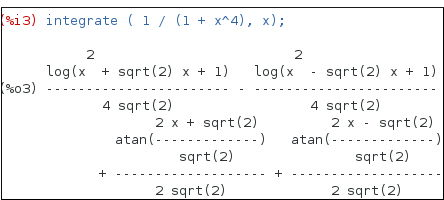
\includegraphics[height= 2cm]{ucarecdn}}
		\uncover<5->{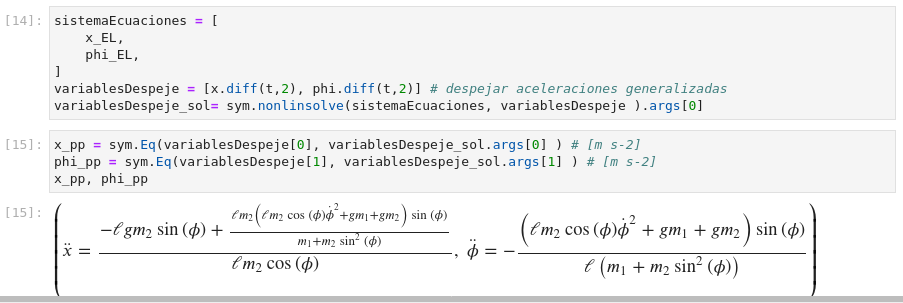
\includegraphics[height= 2cm]{hard}}
\end{frame}


\begin{frame}
	\frametitle{Asistencia docente y corrección asincrónica}
	\begin{block}{Google Colaboratory: comentando y editando el ejercicio del alumno}
		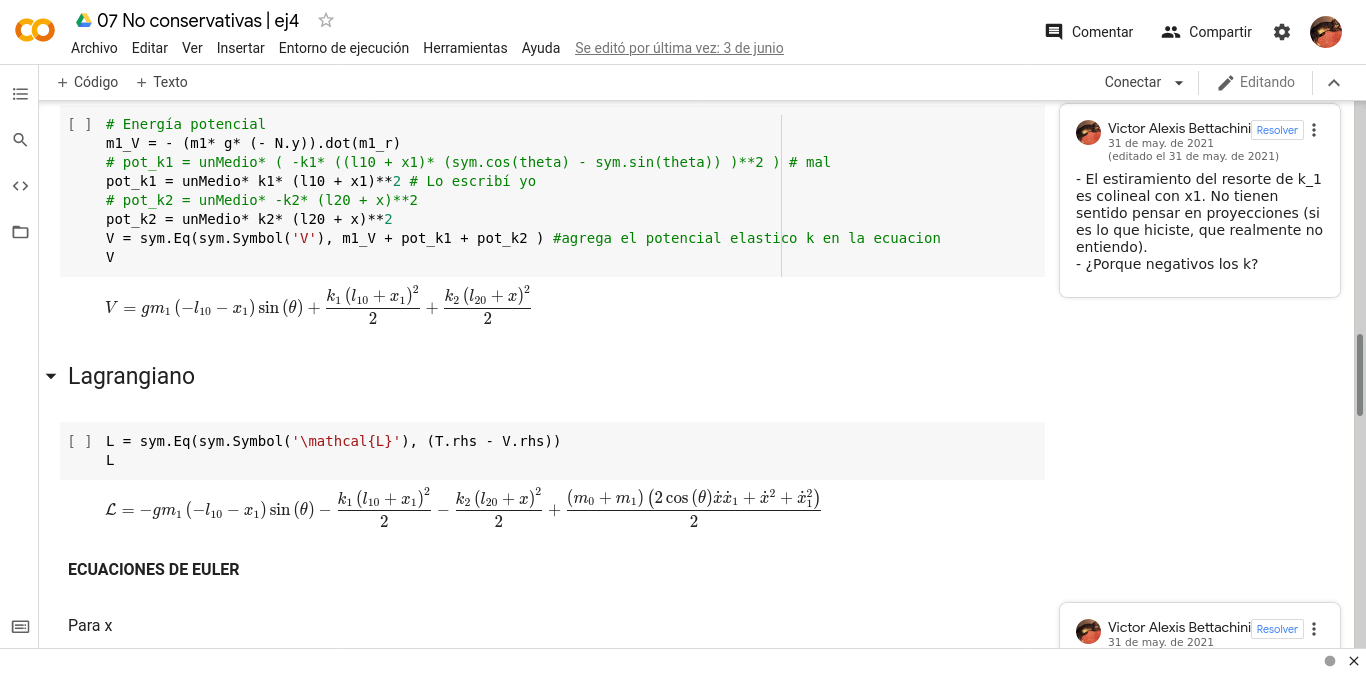
\includegraphics[width= \columnwidth]{comentariosColab}
	\end{block}
\end{frame}


\begin{frame}
	\frametitle{Seguimiento individualizado}
	\begin{block}{Registro del cumplimiento con entregas semanales}
		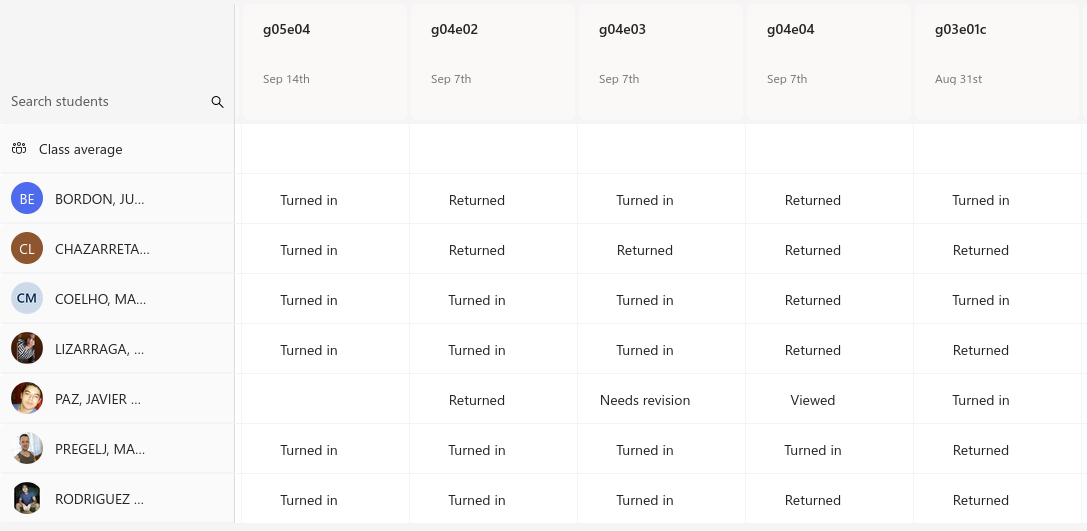
\includegraphics[width= \columnwidth]{seguimiento}
	\end{block}
\end{frame}



\begin{frame}
	\frametitle{Gestión de recursos: tiempo, personal e infraestructura}
  \begin{columns}[b]
    \begin{column}{0.35\textwidth}
			\begin{block}{Aula invertida}
				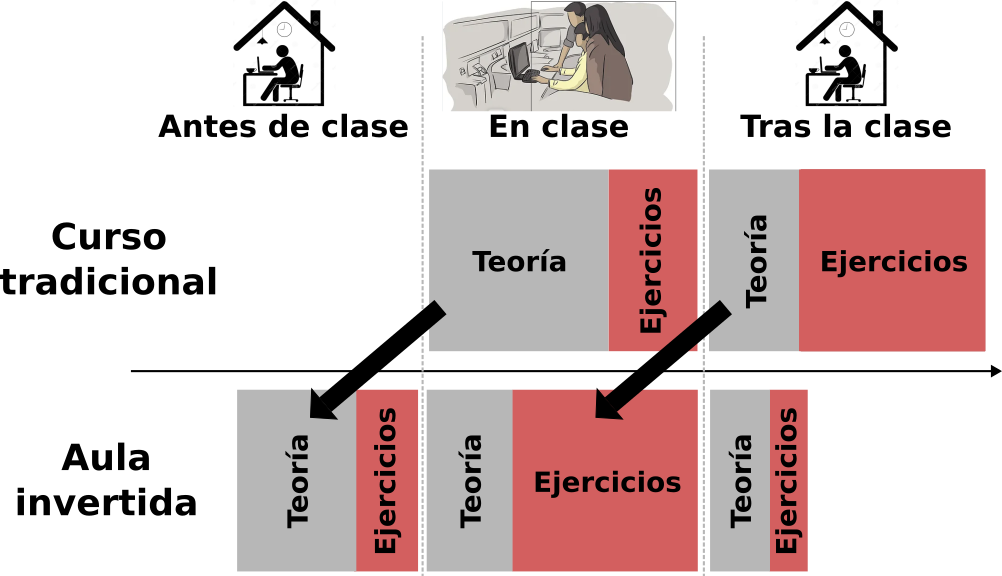
\includegraphics[width= \columnwidth]{diagramaTiempo2.png}
			\end{block}
    \end{column}
    \begin{column}{0.6\textwidth}
			\begin{block}{}
				\begin{tabular}{lll}
					\hline
					Sincrónico & Teoría & Ejercicios\\
					\hline
					Antes & Leer y aplicar & Iniciar\\
					Durante & Aclarar dudas & \begin{tabular}{@{}c@{}}Terminarles\\(semanal)\end{tabular}\\
					Luego & \begin{tabular}{@{}c@{}}Consultas\\adicionales\end{tabular} & \begin{tabular}{@{}c@{}}Correcciones\\del docente\end{tabular}\\
					\hline
				\end{tabular}
			\end{block}
    \end{column}
  \end{columns}
\end{frame}


\begin{frame}
	\frametitle{Pasos futuros}
	\begin{block}{}
 		\begin{description}[<+->]
			\item [Replicar] En 2024 Física II adoptará simulaciones en cuadernos Jupyter.
			\item [Adaptar] Retro-alimentación de los alumnos mejora:
				\begin{itemize}
					\item Apuntes y código en el repositorio.
					\item Metodología de ejercitación y evaluación.
				\end{itemize}
			\item [Actualizar] Incorporar \emph{prompt engineering} a lo enseñado. Que los alumnos exploten sistemas de inteligencia artificial para generar código útil aunque no dominen la sintáxis del lenguaje de programación.
			\item [Difundir] Asesorar y colaborar a quienes quieran incorporar esta metodología en el DIIT.
		\end{description}
	\end{block}
\end{frame}


\end{document}
